\documentclass{VUMIFPSmagistrinis}
% \usepackage{algorithmicx}
% \usepackage{algorithm}
% \usepackage{algpseudocode}
\usepackage{amsfonts}
\usepackage{amsmath}
\usepackage{bm}
\usepackage{caption}
\usepackage{color}
\usepackage{float}
\usepackage{graphicx}
\usepackage{listings}
\usepackage{subfig}
\usepackage{wrapfig}

% Default settings for code listings
\lstset{frame=tb,
  language=scala,
  captionpos=b,
  aboveskip=3mm,
  belowskip=3mm,
  showstringspaces=false,
  columns=flexible,
  basicstyle={\small\ttfamily},
  numbers=none,
  numberstyle=\tiny\color{gray},
  %keywordstyle=\color{blue},
  %commentstyle=\color{dkgreen},
  %stringstyle=\color{mauve},
  frame=single,
  breaklines=true,
  breakatwhitespace=true
  tabsize=3
}

\renewcommand{\lstlistingname}{Kodo pavyzdys}

% Titulinio aprašas
\university{Vilniaus universitetas}
\faculty{Matematikos ir informatikos fakultetas}
\department{Programų sistemų katedra}
\papertype{Magistro baigiamasis darbas}
\title{Programų sistemų kūrimo metodų tyrimas}
\titleineng{Investigation Methods of Software Development}
\author{Vardenis Pavardenis}
% \secondauthor{Vardonis Pavardonis}   % Pridėti antrą autorių
\supervisor{prof. habil. dr. Vardaitis Pavardaitis}
\reviewer{doc. dr. Vardauskas Pavardauskas}
\date{Vilnius – \the\year}

% Nustatymai
% \setmainfont{Palemonas}   % Pakeisti teksto šriftą į Palemonas (turi būti įdiegtas sistemoje)
\bibliography{bibliografija}

\begin{document}
\maketitle

%% Padėkų skyrius
% \sectionnonumnocontent{}
% \vspace{7cm}
% \begin{center}
%     Padėkos asmenims ir/ar organizacijoms
% \end{center}

\sectionnonumnocontent{Santrauka}
Glaustai aprašomas darbo turinys: pristatoma nagrinėta problema ir padarytos
išvados. Santraukos apimtis ne didesnė nei 0,5 puslapio. Santraukų gale
nurodomi darbo raktiniai žodžiai.
% Nurodomi iki 5 svarbiausių temos raktinių žodžių (terminų).
% Vienas terminas gali susidėti iš kelių žodžių.
\raktiniaizodziai{raktinis žodis 1, raktinis žodis 2, raktinis žodis 3, raktinis žodis 4, raktinis žodis 5}

\sectionnonumnocontent{Summary}
Santrauka anglų kalba. Santraukos apimtis ne didesnė nei 0,5 puslapio.
\keywords{keyword 1, keyword 2, keyword 3, keyword 4, keyword 5}

\tableofcontents

\sectionnonum{Įvadas}
Įvade aprašomi darbo tikslai, nurodomas temos aktualumas, aptariamos teorinės
darbo prielaidos bei metodika, apibrėžiamas tiriamasis objektas,
apibūdinami su tema susiję literatūros ar kitokie šaltiniai, temos analizės
tvarka, darbo atlikimo aplinkybės, pateikiama žinių apie naudojamus
instrumentus (programas ir kt.). Darbo įvadas neturi būti dėstymo santrauka.
Įvado apimtis 3-4 puslapiai.

\section{Medžiagos darbo tema dėstymo skyriai}
Išsamiai pateikiamos nagrinėjamos temos detalės: pradiniai duomenys, jų
analizės ir apdorojimo metodai, sprendimų įgyvendinimas, gautų rezultatų
apibendrinimas. Šios dalies turinys labai priklauso nuo darbo temos. Tačiau
visais atvejais joje turi būti tokio pobūdžio skyriai:
\begin{enumerate}
    \item literatūros ar kitokių šaltinių apžvalga. Čia reikėtų daugiau dėmesio
        skirti nuodugnesnėms tam tikros srities studijoms, akademiniams
        strapsniams, įvairių autorių uomonių palyginimui.
    \item analitinė dalis. Šiame skyriuje, nagrinėjant pasirinktą temą ir
        sprendžiant iškeltas problemas, parenkami tyrimo metodai, kurie
        atitiktų ne tik temos pobūdį, bet ir objektyvias tyrėjų galimybes.
        Autorius turi atlikti pakankamai išsamią ir temos turinį
        atskleidžiančią savarankišką analizę;
    \item objekto projektavimas. Šiame skyriuje, integruojant teorines bei
        praktines žinias, aptariamos ir vertinamos galimos sprendimų
        alternatyvos, atskleidžiamas autoriaus siūlomas problemos sprendimo
        kelias, pateikiamas veiksmų planas ar bendrosios jų atlikimo gairės;
    \item objekto realizacija. Aprašoma objekto prototipo realizacija, jo
        savybės, pritaikymo praktikoje galimybės.
\end{enumerate}
Skyriai gali turėti poskyrius ir smulkesnes sudėtines dalis, kaip punktus ir
papunkčius.

\subsection{Kodo pavyzdys}

\begin{lstlisting}[caption=Vartotojo einamosios sąskaitos balansas naudojant įsivaizduojamą Scala API, label=balance][language=Scala]
val duration = 1.weeks
val personalNum = "39008226547"
val balanceStream = Stream(es, "customerBalance")
val notOlderThanOneWeek =
    for {
        event <- balanceStream
        filtered <- event.filter(_.personalNum == personalNum
            && (DateTime.now - _.timeStamp) >= duration)
    } yield filtered
val sum = notOlderThanOneWeek.toList.sum
\end{lstlisting}

\subsection{Poskyris}
Citavimo pavyzdžiai: cituojamas vienas šaltinis \cite{PvzStraipsnLt}; cituojami
keli šaltiniai \cite{PvzStraipsnEn, PvzKonfLt, PvzKonfEn, PvzKnygLt, PvzKnygEn,
PvzElPubLt, PvzElPubEn, PvzMagistrLt, PvzPhdEn}.

\subsubsection{Skirsnis}

\section{Niauroninio tinklo struktūra}
\begin{figure}[H]
    \centering
    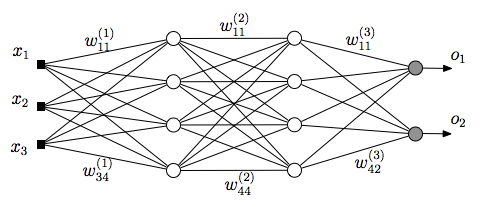
\includegraphics[scale=0.5]{img/MLP}
    \caption{Paveikslėlio pavyzdys}
    \label{img:example}
\end{figure}

\ref{img:example} Paveikslėlio pavyzdys nurodant jį skaičiumi.

\subsubsubsection{Straipsnis}
\subsubsection{Skirsnis}

Kodo pavyzdys:

\section{Skyrius}
\subsection{Poskyris}
\subsection{Poskyris}

\sectionnonum{Rezultatai ir išvados}
Rezultatų ir išvadų dalyje išdėstomi pagrindiniai darbo rezultatai (kažkas
išanalizuota, kažkas sukurta, kažkas įdiegta), pateikiamos išvados (daromi
nagrinėtų problemų sprendimo metodų palyginimai, siūlomos rekomendacijos,
akcentuojamos naujovės).Kaip pavyzdį galima paanalizuoti pelės judėjimo sekimą naudojant Elm kalbą

\printbibliography[heading=bibintoc]  % Šaltinių sąraše nurodoma panaudota
% literatūra, kitokie šaltiniai. Abėcėlės tvarka išdėstomi darbe panaudotų
% (cituotų, perfrazuotų ar bent paminėtų) mokslo leidinių, kitokių publikacijų
% bibliografiniai aprašai. Šaltinių sąrašas spausdinamas iš naujo puslapio.
% Aprašai pateikiami netransliteruoti.

% \sectionnonum{Sąvokų apibrėžimai}
\sectionnonum{Santrumpos}
Sąvokų apibrėžimai ir santrumpų sąrašas sudaromas tada, kai darbo tekste
vartojami specialūs paaiškinimo reikalaujantys terminai ir rečiau sutinkamos
santrumpos.

\appendix  % Priedai
% Prieduose gali būti pateikiama pagalbinė, ypač darbo autoriaus savarankiškai
% parengta, medžiaga. Savarankiški priedai gali būti pateikiami ir
% kompaktiniame diske. Priedai taip pat numeruojami ir vadinami. Darbo tekstas
% su priedais susiejamas nuorodomis.

\section{Niauroninio tinklo struktūra}
\begin{figure}[H]
    \centering
    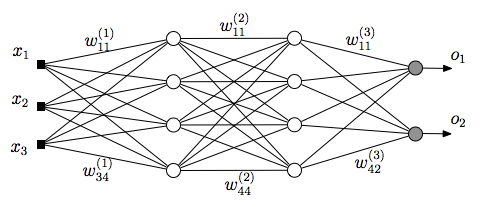
\includegraphics[scale=0.5]{img/MLP}
    \caption{Paveikslėlio pavyzdys}
    \label{img:mlp}
\end{figure}


\section{Eksperimentinio palyginimo rezultatai}
% tablesgenerator.com - converts calculators (e.g. excel) tables to LaTeX
\begin{table}[H]\footnotesize
  \centering
  \caption{Lentelės pavyzdys}
  {\begin{tabular}{|l|c|c|} \hline
    Algoritmas & $\bar{x}$ & $\sigma^{2}$ \\
    \hline
    Algoritmas A  & 1.6335    & 0.5584       \\
    Algoritmas B  & 1.7395    & 0.5647       \\
    \hline
  \end{tabular}}
  \label{tab:table example}
\end{table}

\end{document}
